\documentclass[11pt]{article}
\usepackage[margin=1.5in]{geometry}
\usepackage{graphicx}
\usepackage{float}
\usepackage{parskip}
\usepackage{amsmath}
\usepackage{subfigure}
\usepackage{ulem}
\usepackage{pgfplots}
\pgfplotsset{width=10cm, compat=1.9}

\begin{document}

\textbf{\Huge More On Functions}

Athan Zhang \& Jeffrey Chen

\section{Power and Radical Functions}

A \textbf{power function} is any function of the form $f(x) = ax^{n}$, where $a$ and $n$ are nonzero constant real numbers. 

A \textbf{radical function} is a function that can be written as $f(x) = \sqrt[n]{x^{p}}$, where $n$ and $p$ are positive integers greater than 1 that have no common factors. 

\subsection{Even and Odd Functions}

A function is \textbf{even} if $f(-x) = f(x)$. A function is \textbf{odd} if $f(-x) = -f(x)$. Power functions are the simplest example of this trait: if the power is even, the function is even, and if the power is odd, the function is odd.

\section{Polynomial Functions}


A general polynomial function of degree $n$ can be written in the form:

\[
f(x) = a_nx^n + a_{n-1}x^{n-1} + \ldots + a_1x + a_0
\]

where $a_n, a_{n-1}, \ldots, a_1, a_0$ are the coefficients of the polynomial, and $x$ is the independent variable.

The degree of a polynomial function is the highest power of the variable in the polynomial. For example, the degree of the polynomial function $f(x) = 3x^4 - 2x^2 + 5$ is 4.

% graphs

\subsection{Leading Term Test}

Polynomial functions exhibit various properties and behaviors based on their degree and coefficients. For instance, the \textbf{leading term}, $a_n$, determines the end behavior of the function as $x$ approaches positive or negative infinity. Additionally, the roots of a polynomial function, also known as zeros or solutions, correspond to the values of $x$ where the function equals zero.

\begin{table}[H]
    \centering
    \begin{tabular}{c|c}
        Case & End Behavior \\ \hline
        $a_{n} > 0$, $n$ is odd & $\lim_{x\to -\infty}f(x) = -\infty$ \text{and} $\lim_{x\to \infty}f(x) = \infty$\\
        $a_{n} > 0$, $n$ is even & $\lim_{x\to -\infty}f(x) = \infty$ \text{and} $\lim_{x\to \infty}f(x) = \infty$\\
        $a_{n} < 0$, $n$ is odd & $\lim_{x\to -\infty}f(x) = -\infty$ \text{and} $\lim_{x\to \infty}f(x) = \infty$\\
        $a_{n} < 0$, $n$ is even & $\lim_{x\to -\infty}f(x) = -\infty$ \text{and} $\lim_{x\to \infty}f(x) = -\infty$\\
    \end{tabular}
\end{table}

\subsection{Turning Points}

Turning points indicate where the graph of a function changes from increasing to decreasing and vice versa. Maxima and minima are also located at turning points. 

\begin{center}
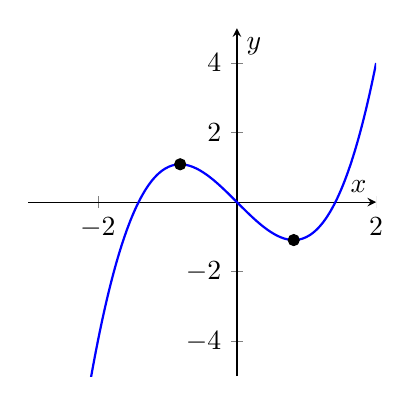
\begin{tikzpicture}
  \begin{axis}[
    xlabel=$x$,
    ylabel=$y$,
    xmin=-3,
    xmax=2,
    ymin=-5,
    ymax=5,
    domain=-3:2,
    samples=100,
    axis lines=middle, width=6cm, height=6cm,
    smooth]

    \addplot[blue, thick] {x^3 - 2*x} node[right] {$f(x) = x^3 - 2x$};

    \addplot[only marks, mark=*] coordinates {(-0.816, 1.089) (0.816, -1.089)};

  \end{axis}
\end{tikzpicture}
\hspace{3em}
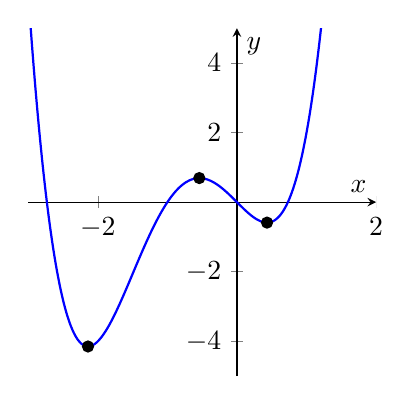
\begin{tikzpicture}
  \begin{axis}[
    xlabel=$x$,
    ylabel=$y$,
    xmin=-3,
    xmax=2,
    ymin=-5,
    ymax=5,
    domain=-3:2,
    samples=100,
    axis lines=middle, width=6cm, height=6cm,
    smooth]

    \addplot[blue, thick] {x^4 + 3*x^3 - 2*x} node[right] {$f(x) = x^4 + 3x^3 - 2x$};

    \addplot[only marks, mark=*] coordinates {(-2.141, -4.148) (-0.541, 0.693) (0.432, -0.587)};

  \end{axis}
\end{tikzpicture}
\end{center}

Notice in the above cubic and quartic functions that the cubic functions have at most 2 turning points and the quartic functions have at most 3 turning points. This pattern can be generalized into the following: \textbf{A polynomial function of degree $n \geq 1$ has at most $n$ distinct real zeros and at most $n - 1$ turning points.}

\subsection{Fundamental Theorem of Algebra}
The Fundamental Theorem of Algebra is a fundamental result in mathematics that establishes the existence and nature of roots for polynomial equations. It states that every non-constant polynomial equation with complex coefficients has at least one complex root.

\textbf{Statement of the Theorem}

Let $P(z)$ be a non-constant polynomial with complex coefficients. Then, the Fundamental Theorem of Algebra states that $P(z)$ can be factored into linear and/or quadratic irreducible factors:
\[ P(z) = a(z - z_1)(z - z_2)\ldots(z - z_n) \]
where $a$ is a non-zero complex constant, $z_i$ are the complex roots of $P(z)$, and $n$ is the degree of the polynomial.

\textbf{Implications}

The Fundamental Theorem of Algebra has several important implications:
\begin{itemize}
  \item Every non-constant polynomial equation of degree $n$ has exactly $n$ complex roots, counting multiplicity.
  
  \item The complex numbers are algebraically closed, meaning that every polynomial equation with complex coefficients has at least one complex root.
  
  \item Real polynomials, which have only real coefficients, can have complex roots as well. Complex roots always occur in conjugate pairs, meaning that if $z$ is a complex root of a real polynomial, then its conjugate $\overline{z}$ is also a root.
  
  \item The degree of a polynomial equation determines the maximum number of roots it can have. For example, a quadratic equation can have at most two distinct roots, a cubic equation can have at most three, and so on.
\end{itemize}

\subsection{Descartes' Rule of Signs}
Descartes' Rule of Signs is a mathematical tool used to determine the possible number of positive and negative real roots of a polynomial equation. It provides a way to efficiently obtain information about the roots without explicitly solving the equation.

\textbf{Statement of the Rule}

Descartes' Rule of Signs states:
\begin{enumerate}
  \item The number of positive real roots of $f(x)$ is either equal to the number of sign changes in the coefficients of $f(x)$ or less than it by an even integer.
  
  \item The number of negative real roots of $f(x)$ is either equal to the number of sign changes in the coefficients of $f(-x)$ or less than it by an even integer.
\end{enumerate}

\textbf{Example:}

Consider the polynomial $f(x) = 3x^4 - 2x^3 + 5x^2 - x - 2$. By examining the coefficients, we count the sign changes:
\[ +, -, +, -, - \]
There are three sign changes, indicating that there are either three positive real roots or one positive real root. To determine the number of negative real roots, we apply the rule to $f(-x)$:
\[ 3(-x)^4 - 2(-x)^3 + 5(-x)^2 - (-x) - 2 \]
\[ +, +, +, +, - \]
There is only one sign change, so there is one negative real root.

Hence, according to Descartes' Rule of Signs, the polynomial $f(x) = 3x^4 - 2x^3 + 5x^2 - x - 2$ has either three or one positive real root, and one negative real root. This rule includes any repeated zeros. 

\section{Zeroes of Polynomial Functions}
The \textbf{zeroes} of a polynomial function refer to the values of $x$ at which the function becomes $0$ or intersects the x-axis. There are many methods to determine these values, some of which will be explained below.

\subsection{Factoring by Grouping}
Students already know how to factor quadratic polynomials, but factoring higher degree polynomials will require some more tricks to master. The first of these is grouping. Grouping is situational and does not work all the time, but is very helpful when it can be used. It is done by "grouping" a polynomial into separate groups, from which each can have a common factor extracted from them. It is easier shown than explained:

Take the polynomial $2x^3 + x^2 + 2x + 1$. Notice two of the terms have a common factor: $2x$. So, we "group" the polynomial in the following way: $(2x^3 + 2x) + (x^2 + 1)$. Next, we factor out the common factor, giving us $2x(x^2 + 1) + (x^2 + 1)$. Finally, the factoring can be completed in an obvious way: $(2x + 1)(x^2 + 1)$.

\subsection{Rational Zeroes Theorem}
The Rational Zeroes Theorem allows us to obtain a list of every possible zero of any polynomial. Let our polynomial of interest have leading term $ax^n$ and constant term $b$. The Rational Zeroes Theorem states that \textbf{every} zero of the polynomial is contained within the list of all combinations of $\frac{f_b}{f_a}$, where $f_b$ is a factor of $b$ and $f_a$ is a factor of $a$. This theorem is a powerful tool for factoring and finding zeroes when used in conjunction with polynomial division, which will be covered in the next section. 

\section{Polynomial Division}
\subsection{Long Division}

Long division of polynomials is a method used to divide one polynomial by another polynomial. It allows us to find the quotient and remainder when dividing polynomials, similar to long division with integers.

To perform long division of polynomials, follow these steps:

\begin{enumerate}
  \item Arrange the dividend (the polynomial to be divided) and the divisor (the polynomial by which we are dividing) in descending order of powers.
  
  \item Divide the leading term of the dividend by the leading term of the divisor to obtain the first term of the quotient.
  
  \item Multiply the entire divisor by the first term of the quotient and subtract it from the dividend. Write the result below the dividend.
  
  \item Bring down the next term from the dividend to create a new dividend.
  
  \item Repeat steps 2-4 until all terms of the dividend have been processed.
  
\end{enumerate}

\subsection{Synthetic Division}

Synthetic division is a shorthand method used to divide a polynomial by a linear binomial of the form $(x - c)$. It provides a quick and efficient way to find the quotient and remainder without having to use long division.

To perform synthetic division, follow these steps:

\begin{enumerate}
  \item Write the coefficients of the polynomial in descending order of powers. If a term is missing, insert a placeholder with a coefficient of zero.
  \item Identify the divisor in the form $(x - c)$ and set $c$ as the divisor. Change the sign of $c$ if necessary.
  \item Draw a horizontal line and write $c$ to the left of it as the synthetic division "divisor."
  \item Bring down the leading coefficient (the coefficient of the highest power term) of the polynomial onto the line.
  \item Multiply $c$ by the number on the line and write the result below the next coefficient. Add the result to that coefficient and write the sum below the line.
  \item Repeat the previous step until all coefficients have been processed.
  \item The number written below the line is the remainder, and the coefficients above the line represent the coefficients of the quotient polynomial.
\end{enumerate}

Here's an example to illustrate the process:

\textbf{Example:} Divide the polynomial $f(x) = 3x^3 - 4x^2 + 2x - 5$ by $(x - 2)$ using synthetic division.

\begin{center}
\begin{tabular}{c|ccccc}
  2 & 3 & -4 & 2 & -5 &\\
    &   & 6 & 4 & 12 & \\
  \hline
  & 3 & 2 & 6 & R:7 \\
\end{tabular}
\end{center}

The remainder is 7, and the coefficients above the line, $2$, $2$, and $6$, represent the coefficients of the quotient polynomial. Therefore, the quotient is $3x^2 + 2x + 6$ with a remainder of $7$. This is written as $3x^2 + 2x + 6 + \frac{7}{x-2}$.

Synthetic division is particularly useful when dividing polynomials with higher degrees and when finding roots (zeros) of a polynomial equation. It simplifies the process and provides a compact representation of the results.

It is important to note that synthetic division can only be used for division by linear binomials of the form $(x - c)$. For division by other types of polynomials, long division or other methods may be required.

\section{Useful Theorems}

\subsection{The Remainder Theorem}

When a function $f(x)$ is divided by a divisor $(x - c)$ with degree 1, the remainder is the real number $r$. So, the division algorithm simplifies to

\begin{align*}
    f(x) = (x - c)\cdot q(x) + r
\end{align*}

Evaluating $f(x)$ for when $x = c$, this becomes

\begin{align*}
    f(c) = (c - c)\cdot q(r) + r = 0 + r = r
\end{align*}

So, $f(c) = r$, which is the remainder. This gives us the \textbf{Remainder Theorem}: 

\begin{center}
\begin{equation*}
\textrm{If a polynomial }  f(x) \, \textrm{is divided by } (x - c), \, \textrm{the remainder is } r = f(c).
\end{equation*}
\end{center}

\subsection{The Factor Theorem}

Using the Remainder Theorem to evaluate $f(x)$ at $x = c$ and the result is $f(c) = 0$, then we know that $c$ is a zero of the function as there is no remainder. This leads us to the \textbf{Factor Theorem}:

\begin{center}
\begin{equation*}
\textrm{A polynomial } f(x) \, \textrm{has a factor } (x - c) \, \textrm{if and only if } f(c) = 0.
\end{equation*}
\end{center}

\section{Rational Functions}

Rational fractions, also known as rational functions, are expressions that represent the quotient of two polynomials. They are a fundamental concept in algebra and provide a powerful framework for studying the relationship between variables.

A rational fraction can be written in the form:

\[
R(x) = \frac{P(x)}{Q(x)},\; Q(x) \neq 0
\]

where $P(x)$ and $Q(x)$ are polynomials, and $Q(x)$ is non-zero.

Rational fractions can exhibit a wide range of behaviors and properties, including the presence of vertical asymptotes, horizontal asymptotes, holes, and critical points.

The key features of rational fractions include:

\begin{itemize}
  \item \textbf{Domain:} The domain of a rational fraction consists of all real numbers except the values of $x$ that make the denominator $Q(x)$ equal to zero. These values are known as the \textit{singularities} of the function.
  \item \textbf{Vertical Asymptotes:} Vertical asymptotes occur at the values of $x$ that make the denominator equal to zero, excluding any common factors with the numerator. 
  \item \textbf{Horizontal Asymptotes:} Horizontal asymptotes describe the behavior of the rational fraction as $x$ approaches positive or negative infinity. If $n$ is the degree of $P(x)$ (the numerator) and $m$ is the degree of $Q(x)$ (the denominator), then the horizontal asymptote is computed as"
  \begin{itemize}
      \item If $n < m$: The horizontal asymptote is $y = 0$
      \item If $n = m$: The horizontal asymptote is $y = \frac{a_{n}}{b_{m}}$ where $a_{n}$ is the coefficient of the highest degree term in the numerator and $b_{m}$ is the coefficient of the highest degree term in the denominator.
      \item If $n + 1 = m $: Their is a slant/oblique asymptote. The function for the oblique asymptote is the remainder polynomial when $P(x)$ is divided by $Q(x)$.
      \item If $n > m$: There is no horizontal asymptote.
  \end{itemize}
  \item \textbf{Holes:} Holes are discontinuities that occur when a factor of the numerator and denominator cancel out. They result in missing points on the graph of the rational function.
\end{itemize}

\section{Nonlinear Inequalities}
Having mastered polynomial and rational functions and equations, it is now time to learn polynomial and rational inequalities. Solving these inequalities will require working with polynomial and rational functions and employing the methods learned in previous sections.

\subsection{Polynomial Inequalities}
Given a polynomial function $f(x)$, a polynomial inequality is of the form $f(x)<0, f(x)\leq 0, f(x)\neq 0, f(x)>0, $ or $f(x)\geq 0$. In these inequalities, intervals for which $f(x)$ is above or below the x-axis are the subjects of interest. In the previous sections, we learned how to find the zeroes of $f(x)$, which will come in handy when finding these intervals of interest. 

In most cases, constructing a \textbf{sign chart} for the polynomial $f(x)$ is sufficient to solve an inequality. This is done by first finding all the zeroes of $f(x)$ and plotting them on a number line. Next, for each interval between zeroes and/or $\pm \infty$, we determine whether $f(x)$ is positive or negative. A completed sign chart can be verified using a graph of the function. Finally, any inequality involving this polynomial can now be solved using the sign chart.

\subsection{Rational Inequalities}
Given a rational function $f(x)$, a rational inequality is of the form $f(x)<0, f(x)\leq 0, f(x)\neq 0, f(x)>0, $ or $f(x)\geq 0$. Similar to polynomial inequalities, these rational inequalities can be solved with a sign chart. However, the construction of a sign chart for a rational function is slightly more complicated.

The first step, like a polynomial sign chart, is plotting points of interest on a number line. However, our points of interest are no longer just zeroes, but are zeroes and singularities. The final step, determining whether f(x) is positive or negative within each interval, is also the same, but requires a little more work. A completed sign chart can be verified using a graph of the function. Finally, any inequality involving this rational function can now be solved using the sign chart.

\section{Partial Fractions}

Partial fractions is a technique used to decompose a rational function into a sum of simpler fractions. It is a powerful tool that allows us to simplify complex expressions and is widely used in algebra and calculus. 

Take a general rational function:

\[
R(x) = \frac{P(x)}{Q(x)}
\]

where $P(x)$ and $Q(x)$ are polynomials, and $Q(x)$ is non-zero.

The goal of partial fractions is to express $R(x)$ as a sum of simpler fractions. This is achieved by decomposing $R(x)$ into partial fractions with denominators that are irreducible (i.e., cannot be factored further).

The process of finding the partial fractions involves the following steps:

\begin{enumerate}
  \item Factor the denominator $Q(x)$ completely into irreducible factors.
  \item Write the partial fraction decomposition as a sum of terms, where each term has a simpler denominator.
  \item Determine the unknown coefficients for each term by comparing the numerators of the original rational function with the decomposition.
\end{enumerate}

There are three main cases for the partial fraction decomposition, depending on the factors of the denominator $Q(x)$:

\begin{enumerate}
  \item \textbf{Distinct Linear Factors:} If $Q(x)$ has distinct linear factors $(x - a)$, the decomposition has terms of the form $\frac{A}{x - a}$, where $A$ is a constant.
  \item \textbf{Repeated Linear Factors:} If $Q(x)$ has repeated linear factors $(x - a)^k$, the decomposition has terms of the form $\frac{A_1}{x - a} + \frac{A_2}{(x - a)^2} + \ldots + \frac{A_k}{(x - a)^k}$, where $A_1, A_2, \ldots, A_k$ are constants.
  \item \textbf{Irreducible Nonlinear Factors:} If $Q(x)$ has an irreducible polynomial factor $S(x)$ of degree $n$, the decomposition has terms of the form $\frac{R(x)}{S(x)}$ where $R(x)$ is a polynomial of degree $n-1$. For example, if there was an irreducible quadratic factor of the form $(ax^2 + bx + c)$, the decomposition has a term of the form $\frac{Ax + B}{ax^2 + bx + c}$, where $A$ and $B$ are constants.
\end{enumerate}

Once the partial fraction decomposition is obtained, it can be used for various purposes, such as simplifying complex algebraic expressions, evaluating limits, taking integrals (both real and complex), determining series expansions, finding inverse Laplace transforms, and more. However, for the purposes of the precalculus course, students do not need to know all the applications of partial fraction decomposition, only how to perform it.

\subsection{Determining Coefficients}
There are multiple ways to determine the coefficients of the terms of the partial fraction decomposition, but the first step regardless of method is to break down the rational function into the terms that will remain using factoring and the rules listed above. For example:

\begin{center}
$\frac{x-1}{x^2+3x+2} = \frac{x-1}{(x+2)(x+1)} = \frac{A}{x+2} + \frac{B}{x+1}$
\end{center}

A more complex example:

\begin{center}
$\frac{x^3+x^2+1}{x^5+x^4-2x^3-x^2-x+2} = \frac{x^3+x^2+1}{(x+2)(x-1)^2(x^2+x+1)} = \frac{A}{x+2} + \frac{B}{(x-1)^2} + \frac{C}{x-1} + \frac{Dx+E}{x^2+x+1}$
\end{center}

Once this step is accomplished, methods to determine the coefficients, represented by capital variables, may be employed.

\subsubsection{Traditional Method}
The traditional method involves creating a system of equations by multiplying by $Q(x)$, the original denominator of the rational function. This eliminates all fractions, leaving us with a more desirable equation. In the case of the first example in the previous section, we are left with:

\begin{center}
$x-1 = A(x+1) + B(x+2)$
\end{center}

Then, we create a system of equations by dividing the new equation by the degree of $x$:

\begin{center}
degree 0: $-1 = A + 2B$ \\
degree 1: $x = Ax + Bx$ \\
$\downarrow$ \\
$A = 3$, $B = -2$
\end{center}

The resulting system may be solved using any number of methods that students should already have under their belts, giving us the coefficients we desire. 

However, this method can be time-consuming, and as the complexity of the problem increases, it can be tedious to use (i.e. the second example from the previous section). So, we will outline another (and often more efficient) method below. Note that for the purposes of precalculus, only the traditional method is necessary to learn.

\subsubsection{Heaviside Cover-Up Method}
Heaviside method provides a quick, easy, and efficient way to determine \textbf{certain} coefficients of partial fractions. To be specific, the coefficients of distinct linear factors and of the highest power terms of repeated linear factors can be found with Heaviside. To illustrate with an example:

\begin{center}
$\frac{x+3}{x^3-3x^2-24x+80} = \frac{x+3}{(x+5)(x-4)^2} = \frac{A}{x+5} + \frac{B}{(x-4)^2} + \frac{C}{x-4}$
\end{center}

Here, $A$ can be found with Heaviside because $x+5$ is a distinct linear factor, and $B$ can be found as well because it is the coefficient of the \textbf{highest power} term of a repeated linear factor, $x-4$. $C$ cannot be found with Heaviside directly, but the process to find it will be greatly simplified through the process. Now, to explain the process of Heaviside. To find an eligible coefficient, follow these steps:

\begin{enumerate}
  \item Look at the original rational function.
  \item Ignore or "cover up" the factor in the denominator to which the coefficient belongs.
  \item Determine what value of $x$ makes that factor $0$.
  \item Plug in that value of $x$ into the "covered up" function.
\end{enumerate}

The resulting value should be the coefficient of interest. To illustrate with an example, let us once again return to the first example from section $7.1$:

\begin{center}
$\frac{x-1}{x^2+3x+2} = \frac{x-1}{(x+2)(x+1)} = \frac{A}{x+2} + \frac{B}{x+1}$
\end{center}

Let us investigate the coefficient $A$ first. It belongs to the factor $x+2$, which is made $0$ by a value of $x=-2$. Next, we look at the original rational function and "cover up" $x+2$:

\begin{center}
$\frac{x-1}{\xout{(x+2)}(x+1)}$
\end{center}

Plugging in our $x$-value of $-2$, we obtain $A = \frac{-3}{-1} = 3$. $B$ can be found with the same process.

Note that in this case, all of our coefficients could be found with Heaviside. Let us investigate an example where this is not the case. Return to the example from earlier in this very section:

\begin{center}
$\frac{x+3}{x^3-3x^2-24x+80} = \frac{x+3}{(x+5)(x-4)^2} = \frac{A}{x+5} + \frac{B}{(x-4)^2} + \frac{C}{x-4}$
\end{center}

As stated before, $A$ and $B$ are eligible for Heaviside: 

\begin{center}
$A = \frac{-5+3}{(-5-4)^2} = -\frac{2}{81}$\\
$B = \frac{4+3}{4+5} = \frac{7}{9}$\\
\end{center}

To find C, we can simply employ the traditional method discussed before. Start by multiplying the equation by the original denominator of the rational function:

\begin{center}
$x+3 = A(x-4)^2 + B(x+5) + C(x+5)(x-4)$\\
$\downarrow$ \\
$x+3 = -\frac{2}{81}(x-4)^2 + \frac{7}{9}(x+5) + C(x+5)(x-4) $
\end{center}

Note that this is a much simpler equation than before due to our efficient elimination of two of the variables using Heaviside. At this point, you may divide the equation into a system based on the degrees of $x$ once again. 

Sometimes, this may still be necessary, but in this case we have no need for a system, considering the fact that only one variable remains. We can simply only consider one of the degrees of $x$. $2$ is the simplest degree to consider here:

\begin{center}
degree 2: $0 = -\frac{2}{81}x^2 + Cx^2$\\
$\downarrow$ \\
$C = \frac{2}{81}$
\end{center}

In conclusion, the Heaviside method cannot be used to determine every coefficient of a partial fraction decomposition, but it can make the process considerably easier and efficient, even for coefficients ineligible for use of the method. 



\end{document}